\section{Rational Non-crossing Partitions}

\begin{definition}[a, b - Non-crossing Partition]
    An \emph{a, b - non-crossing partition} is a tuple
    $(P, Q, f_P, f_Q)$ such that :
    \begin{itemize}
        \item $P \in \mathcal{NC}_{b - 1}$
        \item $Q$ is the Kreweras complement of $P$ : $K(P)$
        \item $\displaystyle \sum_{B \in P}{f_P(B)} + 
                \sum_{B \in Q}{f_Q(B)} = a$
        \item $f_P(B) > \frac{a}{b}$ for each block $B$
                of $P$
        \item $f_Q(B) < \frac{a}{b}$ for each block $B$
                of $Q$
        \item The \emph{rank condition} defined in
                \cite{ref8} holds.
    \end{itemize}
\end{definition}

We denote by $\mathcal{NC}_{a,b}$ the set of 
a, b - non-crossing partitions.

\begin{example}[$a > b : a = 7, b = 3$]
    ~\\
    \begin{center}
        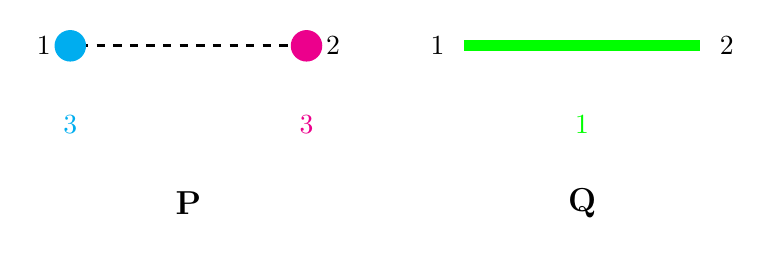
\begin{tikzpicture}[scale=1]
    \node at (1.5,-2) {\large $\mathbf{P}$};
    \node [label = left : {$1$}] (1)
        at (0,0) {};
    \node [label = right : {$2$}] (2)
        at (3,0) {};
    \draw [dashed][very thick] (1) -- (2);
    \fill [color = cyan] (0,0) circle (0.2);
    \fill [color = magenta] (3,0) circle (0.2);
    \node [color = cyan] at (0, -1) {$3$};
    \node [color = magenta] at (3, -1) {$3$};

    \node at (6.5,-2) {\large $\mathbf{Q}$};
    \node [label = left : {$1$}] (1b)
        at (5,0) {};
    \node [label = right : {$2$}] (2b)
        at (8,0) {};
    \draw [color = green][line width = 4pt] (5,0) -- (8,0);
    \node [color = green] at (6.5, -1) {$1$};
  \end{tikzpicture}
    \end{center}
\end{example}

\begin{example}[$a < b : a = 3, b = 5$]
    ~\\
    \begin{center}
        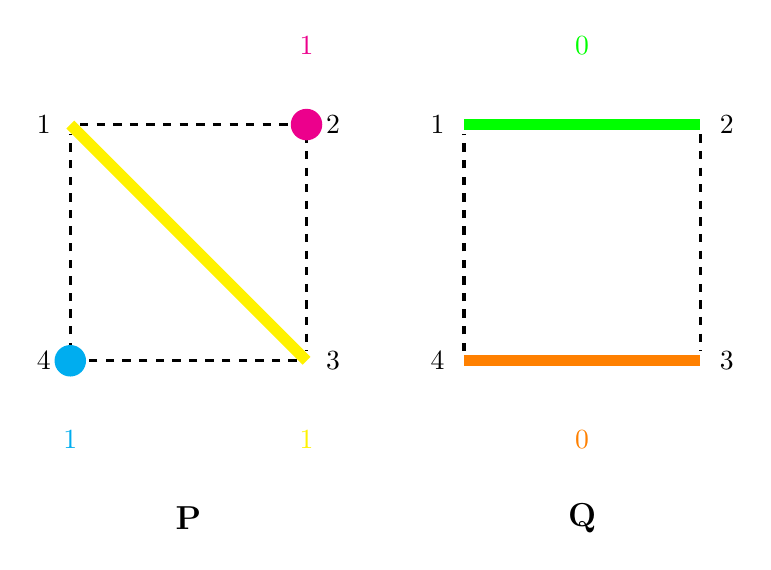
\begin{tikzpicture}[scale=1]
    \node at (1.5,-2) {\large $\mathbf{P}$};
    \node [label = left : {$1$}] (1)
        at (0,3) {};
    \node [label = right : {$2$}] (2)
        at (3,3) {};
    \node [label = right : {$3$}] (3)
        at (3,0) {};
    \node [label = left : {$4$}] (4)
        at (0,0) {};
    \draw [dashed][very thick] (1) -- (2) -- (3) -- (4)
        -- (1);
    \fill [color = cyan] (0,0) circle (0.2);
    \fill [color = magenta] (3,3) circle (0.2);
    \draw [color = yellow][line width = 4pt] (0,3) -- (3,0);
    \node [color = cyan] at (0, -1) {$1$};
    \node [color = magenta] at (3, 4) {$1$};
    \node [color = yellow] at (3, -1) {$1$};

    \node at (6.5,-2) {\large $\mathbf{Q}$};
    \node [label = left : {$1$}] (1b)
        at (5,3) {};
    \node [label = right : {$2$}] (2b)
        at (8,3) {};
    \node [label = right : {$3$}] (3b)
        at (8,0) {};
    \node [label = left : {$4$}] (4b)
        at (5,0) {};
    \draw [dashed][very thick] (1b) -- (2b) -- (3b) -- (4b)
        -- (1b);
    \draw [color = green][line width = 4pt] (5,3) -- (8,3);
    \draw [color = orange][line width = 4pt] (5,0) -- (8,0);
    \node [color = green] at (6.5, 4) {$0$};
    \node [color = orange] at (6.5, -1) {$0$};
  \end{tikzpicture}
    \end{center}
\end{example}

\begin{theorem}[Bodnar, 2017]
    Let $nc_{a,b}$ be the cardinal of $\mathcal{NC}_{a,b}$.
    We have $$nc_{a,b} = \frac{1}{a+b} \binom{a+b}{a} = 
    \frac{(a+b-1)!}{a!b!}$$
\end{theorem}

which is the rational Catalan number $Cat(a,b)$.

\begin{prop}
    This means we can create a \emph{bijection} between
    $\mathcal{PF'}_{a,b}$ and $\mathcal{NC}_{a,b}$.
\end{prop}

\begin{proof}
    Following the proof for the non-primitive case in
    \cite{ref8}, only consider rational Dyck paths where the
    $i^{th}$ North step is labeled $i$.
\end{proof}

\begin{definition}[a, b - Non-crossing 2-Partition]
    An \emph{a, b - Non-crossing 2-partition} is
    a tuple $(P, Q, f_P, f_Q)$ such that :
    \begin{itemize}
        \item $P \in \mathcal{NC}_{b-1}$
        \item $Q$ is the Kreweras complement of $P$ : $K(P)$
        \item $\displaystyle \bigcup_{B \in P}{f_P(B)} \cup
                \bigcup_{B \in Q}{f_Q(B)} = [a]$
        \item $|f_P(B)| > \frac{a}{b}$ for each block $B$
                of $P$
        \item $|f_Q(B)| < \frac{a}{b}$ for each block $B$
                of $Q$
        \item The \emph{rank condition} defined in
            \cite{ref8} holds.  
    \end{itemize}
\end{definition}

This can be seen as a \emph{labeling} of the blocks of
$P$ and $Q$ by $[a]$.

We denote by $\mathcal{NC}^2_{a,b}$ the set of 
a, b - non-crossing 2-partitions.

\begin{example}[$a > b : a = 7, b = 3$]
    ~\\
    \begin{center}
        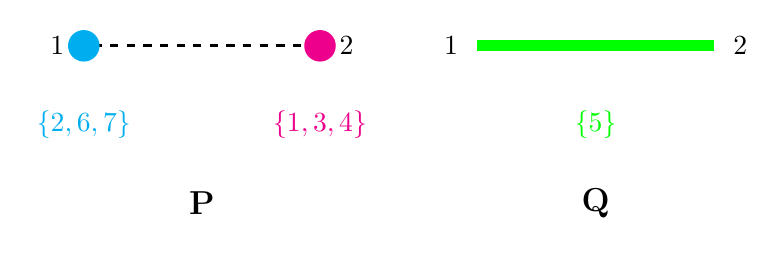
\begin{tikzpicture}[scale=1]
    \node at (1.5,-2) {\large $\mathbf{P}$};
    \node [label = left : {$1$}] (1)
        at (0,0) {};
    \node [label = right : {$2$}] (2)
        at (3,0) {};
    \draw [dashed][very thick] (1) -- (2);
    \fill [color = cyan] (0,0) circle (0.2);
    \fill [color = magenta] (3,0) circle (0.2);
    \node [color = cyan] at (0, -1) {$\{2,6,7\}$};
    \node [color = magenta] at (3, -1) {$\{1,3,4\}$};

    \node at (6.5,-2) {\large $\mathbf{Q}$};
    \node [label = left : {$1$}] (1b)
        at (5,0) {};
    \node [label = right : {$2$}] (2b)
        at (8,0) {};
    \draw [color = green][line width = 4pt] (5,0) -- (8,0);
    \node [color = green] at (6.5, -1) {$\{5\}$};
  \end{tikzpicture}        
    \end{center}
\end{example}

\begin{example}[$a < b : a = 3, b = 5$]
    ~\\
    \begin{center}
        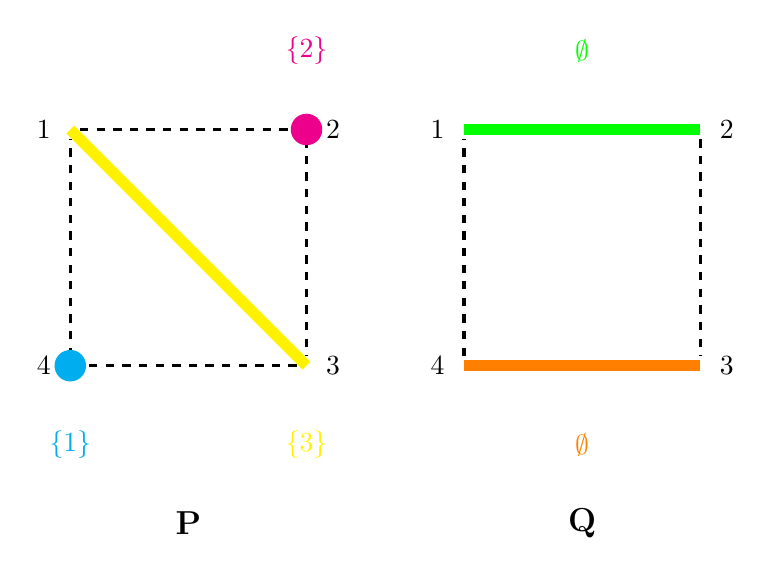
\begin{tikzpicture}[scale=1]
    \node at (1.5,-2) {\large $\mathbf{P}$};
    \node [label = left : {$1$}] (1)
        at (0,3) {};
    \node [label = right : {$2$}] (2)
        at (3,3) {};
    \node [label = right : {$3$}] (3)
        at (3,0) {};
    \node [label = left : {$4$}] (4)
        at (0,0) {};
    \draw [dashed][very thick] (1) -- (2) -- (3) -- (4)
        -- (1);
    \fill [color = cyan] (0,0) circle (0.2);
    \fill [color = magenta] (3,3) circle (0.2);
    \draw [color = yellow][line width = 4pt] (0,3) -- (3,0);
    \node [color = cyan] at (0, -1) {$\{1\}$};
    \node [color = magenta] at (3, 4) {$\{2\}$};
    \node [color = yellow] at (3, -1) {$\{3\}$};

    \node at (6.5,-2) {\large $\mathbf{Q}$};
    \node [label = left : {$1$}] (1b)
        at (5,3) {};
    \node [label = right : {$2$}] (2b)
        at (8,3) {};
    \node [label = right : {$3$}] (3b)
        at (8,0) {};
    \node [label = left : {$4$}] (4b)
        at (5,0) {};
    \draw [dashed][very thick] (1b) -- (2b) -- (3b) -- (4b)
        -- (1b);
    \draw [color = green][line width = 4pt] (5,3) -- (8,3);
    \draw [color = orange][line width = 4pt] (5,0) -- (8,0);
    \node [color = green] at (6.5, 4) {$\emptyset$};
    \node [color = orange] at (6.5, -1) {$\emptyset$};
  \end{tikzpicture}        
    \end{center}
\end{example}

\begin{theorem}[Bodnar, 2017]
    Let $nc^2_{a,b}$ be the cardinal of $\mathcal{NC}^2_{a,b}$.
    We have $$nc^2_{a,b} = b^{a-1}$$.    
\end{theorem}

\begin{prop}
    This means we can create a \emph{bijection} between
    $\mathcal{PF}_{a,b}$ and $\mathcal{NC}^2_{a,b}$.
\end{prop}

\begin{proof}
    See \cite{ref8}.
\end{proof}

While this is an elegant solution, and seems to be the first
to generalize to \emph{all} coprime $a$ and $b$ -- and 
not just those where $a < b$ as studied by Armstrong and others
in the past --, we still wish to define a cover relation for
rational parking functions without having to refer to an other
structure -- especially since this construction makes it even
heavier by having to use rational Dyck paths to verify the
\emph{rank condition} defined in \cite{ref8}.

Therefore, in the next section, we define cover relations
for $\mathcal{PF'}_{a,b}$ and $\mathcal{PF}_{a,b}$ through
(labeled) Rational Dyck Paths, generalizing the classical
case.